%% Table-first extensibility + ObjectNat integration figure (Section 4.2).
%% Standalone TikZ -> tablefirst_figure.pdf. Style matches workflow_figure.tex.
%% Shows: edit edges_gdf with an ordinary GeoPandas mask -> rebuild cached
%% matrix -> the SAME UrbanGraph feeds both IduEdu routing and ObjectNat,
%% with no format conversion.
\documentclass[border=8pt]{standalone}
\usepackage[T1]{fontenc}
\usepackage{helvet}
\renewcommand{\familydefault}{\sfdefault}
\usepackage{array,colortbl}
\usepackage{tikz}
\usetikzlibrary{arrows.meta, positioning, backgrounds, fit, calc}

% ---- palette (shared with workflow_figure) ----
\definecolor{dataBd}{HTML}{475569}\definecolor{dataFl}{HTML}{EEF2F7}
\definecolor{graphBd}{HTML}{0F766E}\definecolor{graphFl}{HTML}{DFF1EE}
\definecolor{downBd}{HTML}{B45309}\definecolor{downFl}{HTML}{FBF0E3}
\definecolor{iduClr}{HTML}{0F766E}
\definecolor{downClr}{HTML}{B45309}
\definecolor{editHi}{HTML}{FBE3C3}
\definecolor{hdrGray}{HTML}{E4E9EF}
\definecolor{bandFl}{HTML}{FCF6EE}
\definecolor{bandBd}{HTML}{E0B583}

\newcommand{\hd}{\small\bfseries}

\begin{document}
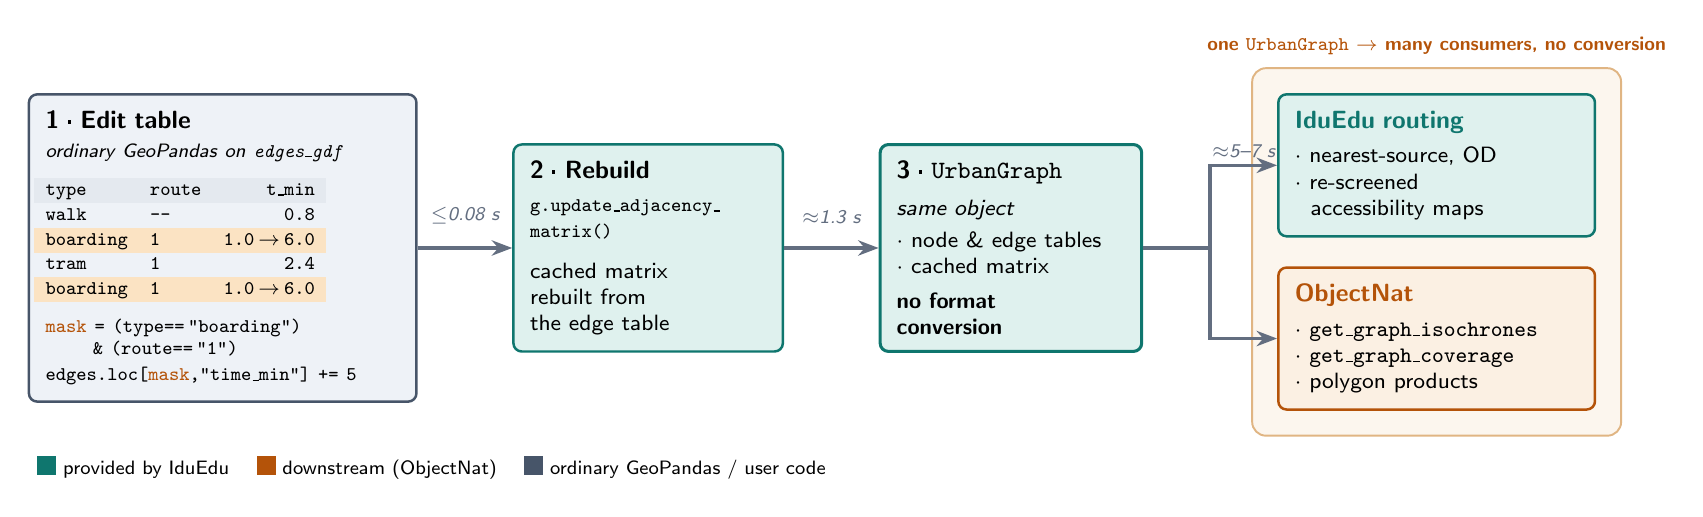
\begin{tikzpicture}[
  font=\footnotesize,
  >={Stealth[length=2.6mm]},
  stage/.style={rounded corners=3pt, draw, line width=0.9pt, align=left,
                inner sep=6pt, anchor=north},
  flow/.style={->, line width=1.2pt, draw=dataBd!85},
  ann/.style={font=\scriptsize\itshape, text=dataBd!85, align=center},
]

% ---------- A: edit table (ordinary GeoPandas) ----------
\node[stage, draw=dataBd, fill=dataFl, text width=4.5cm] (A) at (0,0) {%
  {\hd 1~\textperiodcentered~Edit table}\\[1pt]
  {\scriptsize\itshape ordinary GeoPandas on \texttt{edges\_gdf}}\\[5pt]
  {\ttfamily\scriptsize
  \setlength{\tabcolsep}{4pt}\renewcommand{\arraystretch}{1.12}
  \begin{tabular}{@{}ll r@{}}
    \rowcolor{hdrGray} type & route & t\_min\\
    walk & -- & 0.8\\
    \rowcolor{editHi} boarding & 1 & 1.0$\,\to\,$6.0\\
    tram & 1 & 2.4\\
    \rowcolor{editHi} boarding & 1 & 1.0$\,\to\,$6.0\\
  \end{tabular}}\\[5pt]
  {\ttfamily\scriptsize\textcolor{downClr}{mask} = (type==\,"boarding")\\
  \hspace*{6mm}\& (route==\,"1")\\
  edges.loc[\textcolor{downClr}{mask},"time\_min"] += 5}
};

% ---------- B: rebuild cached matrix ----------
\node[stage, draw=graphBd, fill=graphFl, text width=3.0cm, right=1.2cm of A] (B) {%
  {\hd 2~\textperiodcentered~Rebuild}\\[4pt]
  {\ttfamily\scriptsize g.update\_adjacency\_\\ matrix()}\\[5pt]
  cached matrix\\ rebuilt from\\ the edge table
};

% ---------- C: the same UrbanGraph object ----------
\node[stage, draw=graphBd, fill=graphFl, line width=1.1pt, text width=2.9cm,
      right=1.2cm of B] (C) {%
  {\hd 3~\textperiodcentered~\texttt{UrbanGraph}}\\[4pt]
  {\itshape same object}\\[2pt]
  $\cdot$ node \& edge tables\\
  $\cdot$ cached matrix\\[3pt]
  \textbf{no format} \\ \textbf{conversion}
};

% ---------- D1 / D2: two consumers of the same object ----------
\node[stage, draw=graphBd, fill=graphFl, text width=3.6cm, anchor=west]
      (D1) at ($(C.east)+(1.7cm,1.05cm)$) {%
  {\hd\textcolor{iduClr}{IduEdu routing}}\\[3pt]
  $\cdot$ nearest-source, OD\\
  $\cdot$ re-screened\\ \hspace*{2mm}accessibility maps
};

\node[stage, draw=downBd, fill=downFl, text width=3.6cm, anchor=west]
      (D2) at ($(C.east)+(1.7cm,-1.15cm)$) {%
  {\hd\textcolor{downClr}{ObjectNat}}\\[3pt]
  $\cdot$ \texttt{get\_graph\_isochrones}\\
  $\cdot$ \texttt{get\_graph\_coverage}\\
  $\cdot$ polygon products
};

% ---------- forward flow ----------
\draw[flow] (A) -- (B);
\draw[flow] (B) -- (C);
\coordinate (fork) at ($(C.east)+(0.85cm,0)$);
\draw[line width=1.2pt, draw=dataBd!85] (C.east) -- (fork);
\draw[flow] (fork) |- (D1.west);
\draw[flow] (fork) |- (D2.west);

% ---------- arrow timing annotations ----------
\node[ann, above=1pt] at ($(A.east)!0.5!(B.west)+(0,0.15)$) {$\le$0.08~s};
\node[ann, above=1pt] at ($(B.east)!0.5!(C.west)+(0,0.15)$) {$\approx$1.3~s};
\node[ann, anchor=south] at ($(fork)!0.5!(D1.west)+(0,0.5cm)$) {$\approx$5--7~s};

% ---------- band over the two consumers ----------
\begin{scope}[on background layer]
  \node[rounded corners=5pt, fill=bandFl, draw=bandBd, line width=0.7pt,
        fit=(D1)(D2), inner sep=9pt] (band) {};
\end{scope}
\node[anchor=south, downClr, font=\scriptsize\bfseries]
  at ($(band.north)+(0,1pt)$)
  {one \texttt{UrbanGraph} $\rightarrow$ many consumers, no conversion};

% ---------- legend ----------
\node[anchor=north west, font=\scriptsize] at ($(A.south west)+(0,-0.55cm)$) {%
  \textcolor{iduClr}{\rule{2.4mm}{2.4mm}}~provided by IduEdu \quad
  \textcolor{downClr}{\rule{2.4mm}{2.4mm}}~downstream (ObjectNat) \quad
  \textcolor{dataBd}{\rule{2.4mm}{2.4mm}}~ordinary GeoPandas / user code};

\end{tikzpicture}
\end{document}
